 \documentclass[a4paper, 12pt,oneside]{article}
\usepackage{graphicx} % Required for inserting images
\usepackage[top=2.5cm, bottom=2cm, left=2cm, right=2cm]{geometry}
\usepackage[french]{babel}  % Définit le français comme langue principale
\usepackage[utf8]{inputenc}  % Gère les accents et caractères spéciaux (si nécessaire)
\usepackage[T1]{fontenc}
\usepackage[colorlinks,bookmarks=false,linkcolor=black,urlcolor=blue, citecolor=black]{hyperref}
\usepackage{units}
\usepackage{verbatim}
\usepackage{verbdef}% http://ctan.org/pkg/verbdef
\usepackage{amsmath}
\usepackage{amssymb}
\usepackage{wrapfig}
\usepackage{subcaption}
\usepackage{caption}
\usepackage{float}
\usepackage[export]{adjustbox}
\usepackage{upgreek}
\usepackage{hyperref}
%Pour changer la taille des titres de section et subsection. Ajoutez manuellement les autres styles si besoin.
\makeatletter
\renewcommand{\section}{\@startsection {section}{1}{\z@}%
             {-3.5ex \@plus -1ex \@minus -.2ex}%
             {2.3ex \@plus.2ex}%
             {\normalfont\normalsize\bfseries}}
\makeatother

\makeatletter
\renewcommand{\subsection}{\@startsection {subsection}{1}{\z@}%
             {-3.5ex \@plus -1ex \@minus -.2ex}%
             {2.3ex \@plus.2ex}%
             {\normalfont\normalsize\bfseries}}
\makeatother

\graphicspath{{Graphes/}}

\begin{document}
\title{\normalsize{Lab Work Report - Group N$^\circ$\\ XX - Experiment}}
\date{\normalsize{\today}}
\author{\normalsize{Name} 1\and \normalsize{Name 2}}

\begin{center}
\large\textbf{\sffamily Expérience N$^\circ$D3. Plasticité des solides}\\%
\large\sffamily Groupe N$^\circ$22: Armand Le Douarec, Maxime Chatelin\\%
\large\sffamily\today\quad   Assistant -  Max Lo Conte \\%
\end{center}

\section{Introduction}
\vspace{-0.2cm}

La plasticité des métaux, étudiée depuis l’Antiquité avec le passage de l’âge de pierre à l’âge du bronze [\ref{ref1}], demeure un sujet crucial pour les applications industrielles modernes. La capacité d’un matériau à se déformer plastiquement sans se rompre a permis de concevoir des objets durables, depuis les premiers outils en bronze jusqu’aux structures avancées en alliages métalliques utilisées en aéronautique [\ref{ref2}] ou en automobile [\ref{ref3}]. Grâce à des traitements thermiques adaptés, il est possible de modifier la dureté et la malléabilité des métaux, optimisant ainsi leurs propriétés mécaniques en fonction des usages. Ce travail pratique se propose d’étudier la plasticité d’un alliage d’aluminium industriel, l’Anticorodal 110 [\ref{ref4}], en soumettant plusieurs échantillons à différents traitements thermiques. Par le biais d’essais de traction, nous déterminerons les propriétés mécaniques essentielles de cet alliage, notamment le module de Young, la limite élastique, la résistance mécanique à la traction et la déformation à la rupture, afin de mieux comprendre l’impact de ces traitements sur sa résistance et sa ductilité.

\vspace{-0.2cm}
\section{Théorie}
\vspace{-0.2cm}

\paragraph{Déformation élastique et plastique}

\begin{wrapfigure}{h}{0.2\textwidth}
    \vspace{-0.8cm}
    \centering
    \includegraphics[width=1\linewidth]{déformation_plastique.png}
    \captionsetup{justification=centering}
    \caption{Mouvement d'une déformation plastique dans un cristal [\ref{ref5}]}
    \label{fig1}
    \vspace{2cm}
\end{wrapfigure}

Quand un solide subit une contrainte extérieure, soit il se déplace, soit il se déforme selon l’intensité de la force exercée. Dans le deuxième cas, sous une faible contrainte, la déformation est proportionnelle à la contrainte, selon la loi de Hooke, exprimée par la relation [\ref{ref5}] :

\vspace{-0.5cm}
\begin{equation}
    \sigma=E\,\varepsilon.
\label{eq1}
\end{equation}
\vspace{-0.4cm}

\noindent où $\sigma$ représente la contrainte appliquée, $E$ est le module de Young, et $\varepsilon$ est la déformation induite. 

Ce phénomène, appelé déformation élastique, peut être expliqué par l'élasticité des liaisons atomiques, et est réversible : la forme initiale du solide est entièrement retrouvée lorsque la contrainte disparaît. En revanche, si la contrainte dépasse une certaine limite, dite limite élastique, alors, la relation de proportionnalité ne tient plus. Vient alors la déformation plastique, qui résulte d’une modification irréversible de la structure atomique du solide, principalement par le glissement des plans atomiques sous l’effet d’une contrainte de cisaillement comme montré sur la Fig.(\ref{fig1}). Ce phénomène est causé par le mouvement de défauts dans le réseau cristallin, appelés dislocations, qui se déplacent le long des plans de glissement. Les dislocations permettent ainsi au matériau de se déformer sans rupture immédiate, un mécanisme essentiel pour la malléabilité des métaux [\ref{ref5}].

\vspace{-0.2cm}
\paragraph{Essai de traction}

Une méthode courante pour analyser les propriétés plastiques des matériaux est l’essai de traction. Ce test permet de mesurer leur comportement sous une contrainte croissante. Ce test consiste à appliquer une force de traction à vitesse constante sur une éprouvette, permettant d’observer l’évolution de la force $F$ en fonction de l’allongement $\Delta l$ de l’échantillon. En utilisant les relations suivantes [\ref{ref5}]:

\begin{equation}
    \sigma = \frac{F}{S_0} \quad \quad \quad \varepsilon = \frac{\Delta l}{l_0}
\label{eq1}
\end{equation}

\noindent 
avec $S_0$  la section initiale de l’échantillon et $l_0$ sa longueur initiale. \\

\begin{wrapfigure}{h}{0.4\textwidth}
    \centering
    \includegraphics[width=1\linewidth]{courbe_conv_metal.png}
    \captionsetup{justification=centering}
    \caption{Courbe de traction conventionnelle d'un métal [\ref{ref5}]}
    \label{fig2}
\end{wrapfigure}

La Fig.(\ref{fig2}) trace la courbe de la contrainte $\sigma$ en fonction de la déformation $\varepsilon$, aussi appelée courbe de traction. Cette courbe est divisée en trois zones : (I) le domaine élastique, où la déformation est proportionnelle à la contrainte et réversible ; (II) le domaine plastique, où la déformation devient irréversible, laissant une trace résiduelle dans le matériau ; et (III) la striction, une déformation plastique localisée qui précède la rupture. Les points clés de la courbe incluent la limite élastique $\sigma_{0.2}$, la résistance mécanique à la traction $\sigma_{\text{max}}$, ainsi que la déformation à la rupture $\varepsilon_{\text{rup}}$.

Définir précisément la limite élastique $\sigma_0$ est théoriquement possible mais délicat en pratique, car les premières déformations plastiques sont infimes et difficiles à discerner, notamment en raison des défauts internes du matériau. Pour simplifier cette mesure, la contrainte $\sigma_{0.2}$, correspondant à une déformation plastique résiduelle de 0,2\,\%, est utilisée comme approximation fiable de la transition élastique-plastique. Enfin, le module de Young $E$ est défini comme la pente de la courbe dans le domaine élastique.

\paragraph{Durcissement d'un d'alliage}

Le durcissement des alliages repose sur l'interaction des dislocations avec des précipités, des groupements d'atomes étrangers présents dans le métal. Ces précipités peuvent être des éléments d'alliage dissous dans la matrice métallique, formant des structures qui entravent le mouvement des dislocations (Fig.(\ref{fig3})), ce qui augmente la limite élastique. En bloquant ces dernières, les précipités augmentent la résistance du matériau à la déformation plastique. À l'inverse, pour adoucir un alliage et faciliter sa déformation, on peut dissoudre ces précipités en chauffant le métal à une température où leur solubilité est plus élevée, et n'étant plus un frein aux déformations plastiques, rend la structure métallique plus malléable.

\begin{figure}[H]
    \centering
    \includegraphics[width=0.45\textwidth]{blocage_déformation.png}
    \captionsetup{justification=centering}
    \caption{Schéma de blocage des déformations plastiques par les précipités [\ref{ref5}]}
    \label{fig3}
\end{figure}

\section{Démarche expérimentale}

Ces expériences vont permettre de mettre en lumière les propriétés de l'alliage d'aluminium industriel Al\,-\,0.7\%Si, connu sous le nom d'Anticorodal 110 [\ref{ref4}]. Les essais sont réalisés sur six échantillons de cet alliage, soumis à différents traitements thermiques: Les deux premiers échantillons sont testés dans leur état initial, sans aucun traitement thermique préalable. Les quatre autres échantillons sont chauffés dans un four à $(550 \pm 5)$\,°C pendant 1 heure. Après ce chauffage, ils sont rapidement refroidis en les plongeant dans de l'eau à température ambiante. Deux échantillons sont ensuite testés immédiatement après le refroidissement. Les deux échantillons restants subissent un second chauffage à $(250 \pm 5)$\,°C pendant 20 minutes. Ces échantillons sont également refroidis dans de l'eau à température ambiante après chaque chauffage, puis soumis aux tests de traction. Chaque condition thermique est testée sur deux échantillons pour minimiser les risques d’erreur pendant les essais.
Les tests de traction sont effectués à l’aide d’une machine de traction. Les échantillons sont fixés dans la machine à l’aide de vis de serrage, et un capteur de déformation est attaché à chaque échantillon pour mesurer son allongement pendant l’essai. La machine tire les extrémités de l’échantillon à vitesse constante, et les tensions générées sont enregistrées sur un ordinateur. La force est obtenue à partir des tensions mesurées par le capteur de force, avec une sensibilité de $0.002$\,MPa en prenant en compte l'effet de levier, tandis que la déformation est mesurée par le capteur de déformation avec une sensibilité de $0.2$\,V/mm. L'aire de la section transversale $S_0$ et la longueur entre les vis $l_0$ sont mesurées pour chaque échantillon avant de réaliser l'essai de traction.

\section{Résultats}

Le premier échantillon, qui a été testé dans son état initial, présente les caractéristiques suivantes : une longueur initiale $l_0 = (18.20 \pm 0.005)$\,mm et une aire de section transversale $S_0 = (8.08 \pm 0.08)$\,mm$^2$. Toutes les figures suivantes présentent la contrainte $\sigma$ en fonction de l'allongement relatif $\varepsilon$ d'un échantillon. La Fig.(\ref{fig4}) présente la courbe de traction d'un des deux échantillons non traités. Le deuxième échantillon non traité n'a pas donné de retours concluants, avec un module de Young négatif et a donc été négligé, mais son graphe est disponible en annexe.
\vspace{-0.8cm}
\begin{figure}[H]
    \centering
    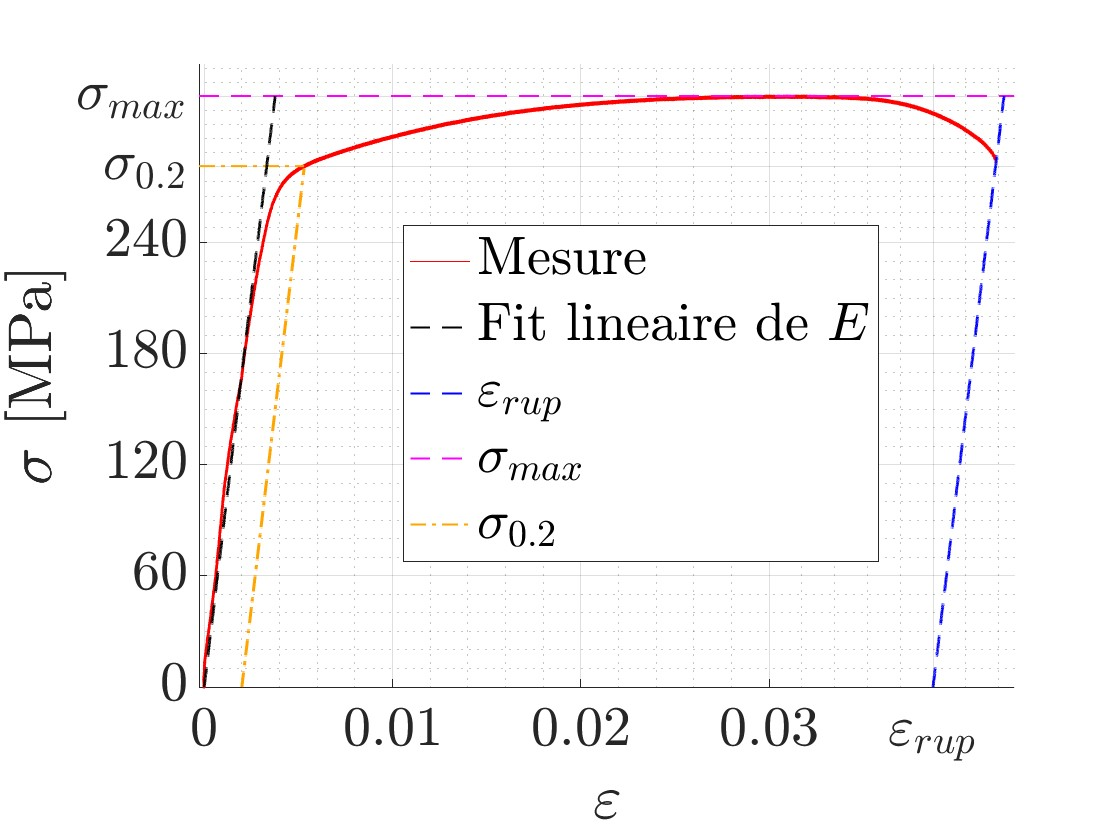
\includegraphics[width=0.45\textwidth]{GRAPHES/Graphe_1.jpg}
    \captionsetup{justification=centering}
    \caption{Courbe de traction du premier échantillon non traité}
    \label{fig4}
\end{figure}
\vspace{-1cm}
\begin{figure}[H]
    \centering
    \begin{minipage}{0.45\textwidth}
        \centering
        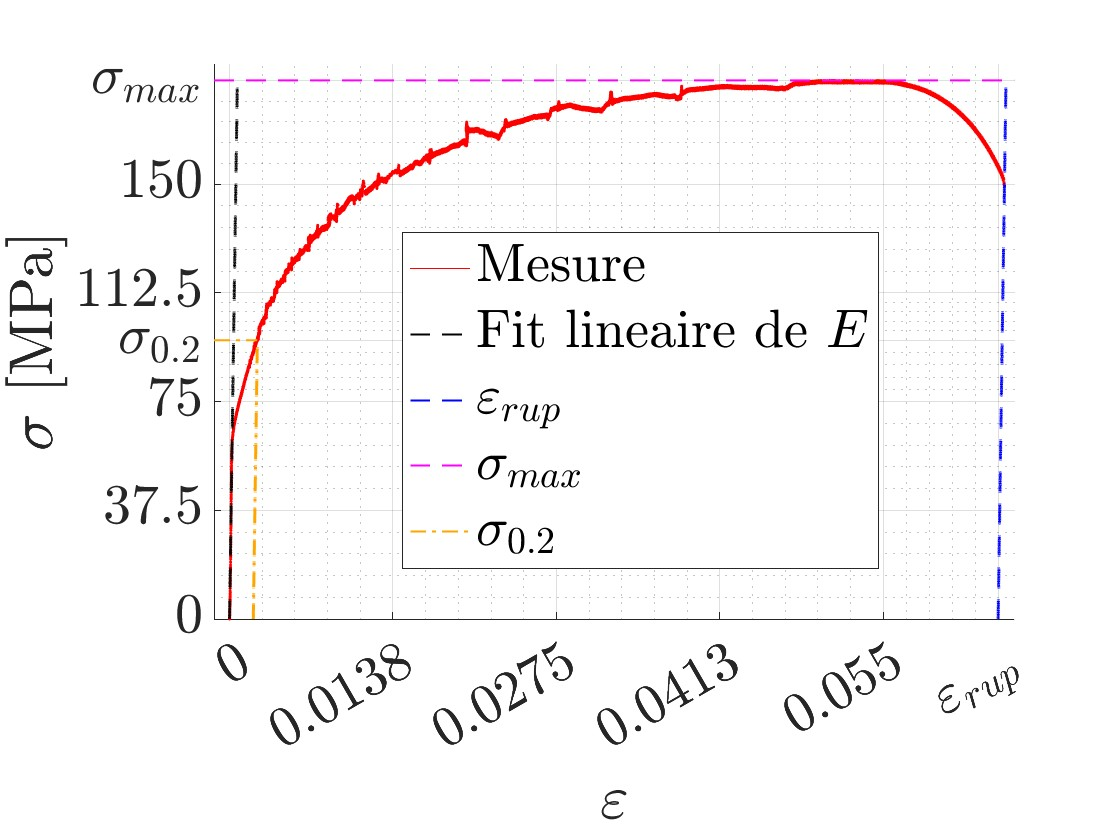
\includegraphics[width=\linewidth]{GRAPHES/Graphe_4.jpg}
        \captionsetup{justification=centering}
        \caption{Courbe de traction du premier échantillon chauffé à $(550 \pm 5 )$\,°C pendant 1 heure.}
        \label{fig5}
    \end{minipage}
    \hfill
    \begin{minipage}{0.45\textwidth}
        \centering
        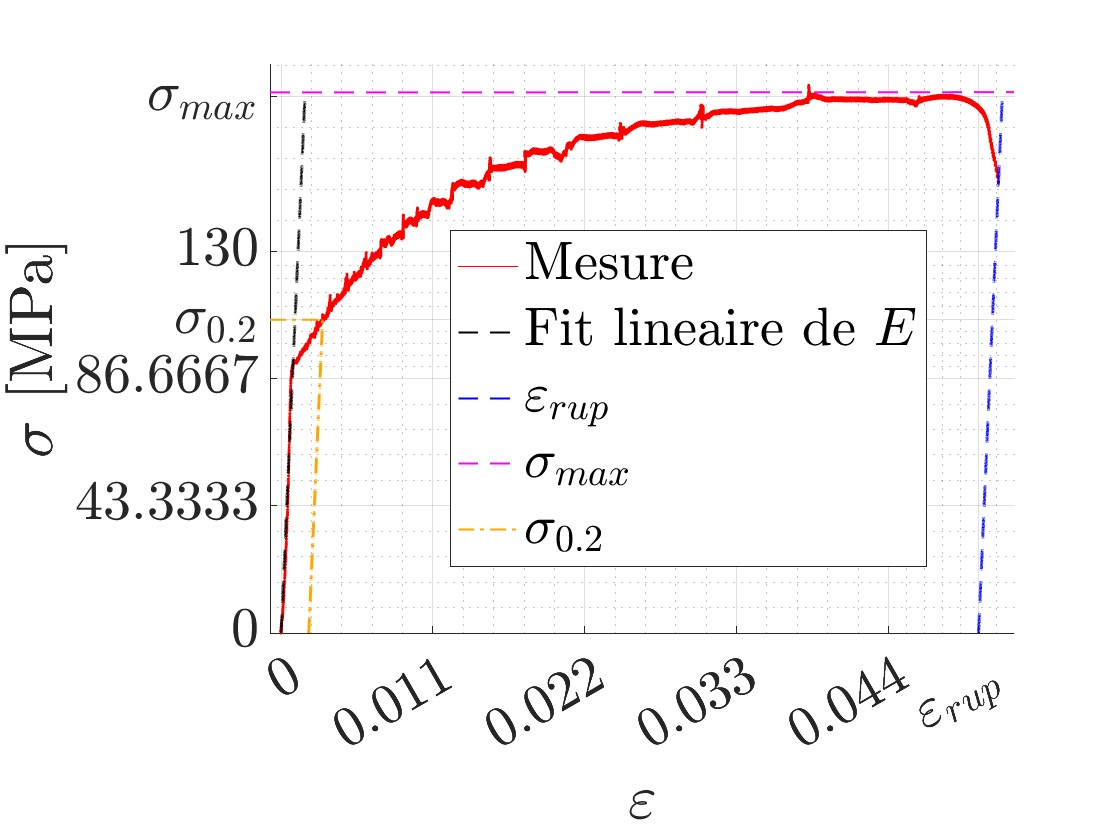
\includegraphics[width=\linewidth]{GRAPHES/Graphe_3.jpg}
        \captionsetup{justification=centering}
        \caption{Courbe de traction du deuxième échantillon chauffé à $(550 \pm 5 )$\,°C pendant 1 heure}
        \label{fig6}
    \end{minipage}
\end{figure}

Le premier échantillon chauffé dans un four pendant une heure à $(550 \pm 5)$\,°C a une longueur initiale de $l_0 = (19.14 \pm 0.005)$\,mm, une aire de section transversale de $S_0 = (8.08 \pm 0.08)$\,mm$^2$ et sa courbe de traction est présente dans la Fig.(\ref{fig5}). Le deuxième échantillon ayant subi le même traitement thermique possède une longueur initiale $l_0 = (18.54 \pm 0.005)$\,mm et une section $S_0 = (7.97 \pm 0.14)$\,mm$^2$. Sa courbe de traction est représentée dans la Fig.(\ref{fig6}) \\


Enfin, pour les échantillons réchauffés pendant 20 minutes à $(250 \pm 5)$\,°C après avoir initialement été chauffés à $(550 \pm 5)$\,°C pendant une heure, le premier échantillon possède une longueur initiale de $l_0 = (18.04 \pm 0.005)$\,mm et une aire de section transversale de $S_0 = (8.06 \pm 0.14)$\,mm$^2$. Le second a pour longueur initiale une longueur $l_0 = (18.34 \pm 0.005)$\,mm et une aire de section transversale $S_0 = (8.2 \pm 0.2)$\,mm$^2$. Les Fig.(\ref{fig7}) et Fig.(\ref{fig8}) montrent respectivement les courbes de traction du premier et deuxième échantillon ayant subi deux traitements thermiques distincts.

\begin{figure}[H]
    \centering
    \begin{minipage}{0.45\textwidth}
        \centering
        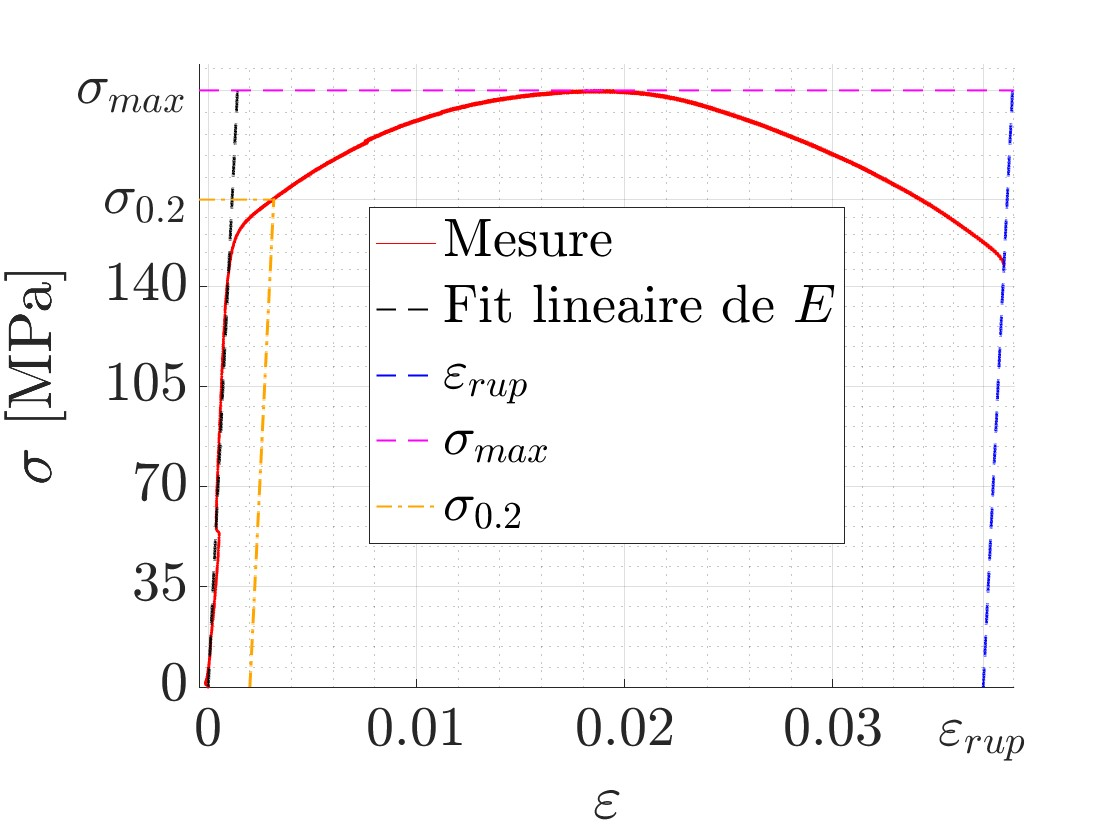
\includegraphics[width=\linewidth]{GRAPHES/Graphe_6.jpg}
        \captionsetup{justification=centering}
        \caption{Courbe de traction du premier échantillon chauffé à $(550 \pm 5)$\,°C pendant 1 heure, thermalisé à température ambiante puis chauffé de nouveau à $(250 \pm 5)$\,°C pendant 20 minutes}
        \label{fig7}
    \end{minipage}
    \hfill
    \begin{minipage}{0.45\textwidth}
        \centering
        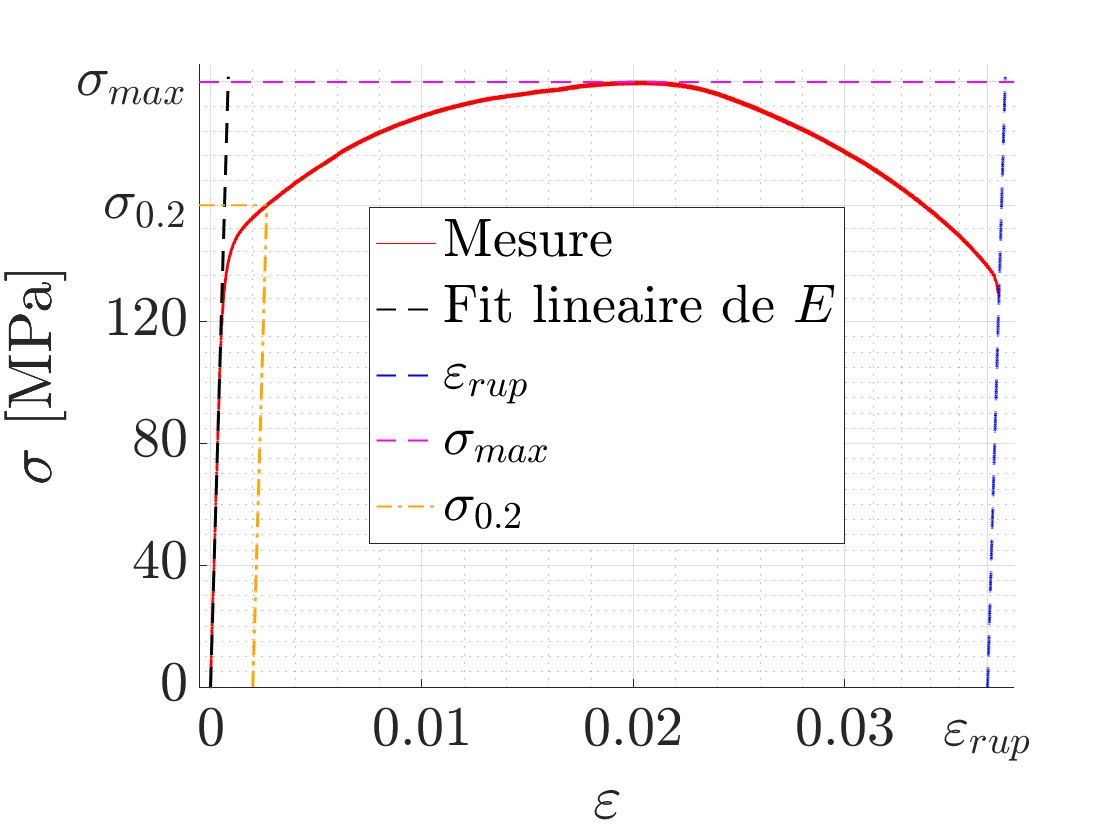
\includegraphics[width=\linewidth]{GRAPHES/Graphe_5.jpg}
        \captionsetup{justification=centering}
        \caption{Courbe de traction du second échantillon chauffé à $(550 \pm 5)$\,°C pendant 1 heure, thermalisé à température ambiante puis chauffé de nouveau à $(250 \pm 5)$\,°C pendant 20 minutes}
        \label{fig8}
    \end{minipage}
\end{figure}

Il est important de noter que ces courbes de traction ont été ajustées en ajoutant des offsets horizontaux et verticaux lorsque nécessaire afin que le début des graphes corresponde à l'origine du repère. Cela permet de garantir que les valeurs extraites des graphes sont correctement alignées et représentatives des données obtenues lors des tests. 

La Fig.(\ref{fig9}) ci-dessous montre une superposition des courbes de traction de trois échantillons 'A' (voir Tab.(\ref{tab1})) ayant subis trois traitements thermiques différents et le Tab.(\ref{tab1}) expose les valeurs $E$, $ \sigma_{0.2}$, $\sigma_{max}$ et $\varepsilon_{rup}$ pour chacun des échantillons ainsi que leur section $S_0$. Le Tab.(\ref{tab2}) montre les valeurs de référence ou du moins les valeurs minimales attendues pour ces quatre grandeurs déterminées à partir des courbes de traction pour l'échantillon d'Anticorodal-110 non chauffé d'épaisseur $e=(2.00 \pm 0.005)$\,mm. Cela permet d'obtenir les erreurs relatives des mesures effectuées dans ce TP.

\begin{figure}[H]
    \centering
    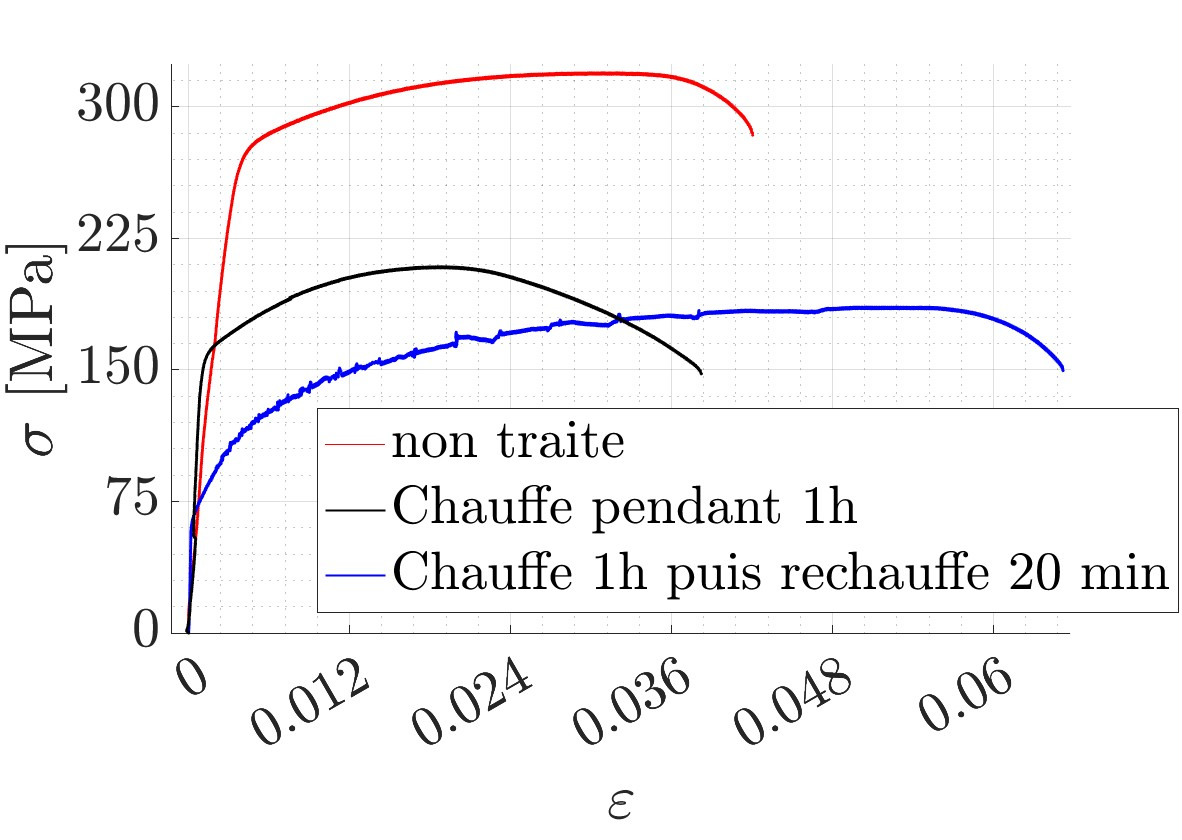
\includegraphics[width=0.45\textwidth]{GRAPHES/Graphe_7_bis.jpg}
    \captionsetup{justification=centering}
    \caption{Courbes de traction des trois échantillons 'A' ayant subi divers traitements thermiques}
    \label{fig9}
\end{figure}

\vspace{-0.5cm}

\begin{table}[H]
\centering
\begin{tabular}{|c|c|c|c|c|c|}
\hline
Échantillon & \( S_0 \, [\text{mm}^2] \) & \( E \, [\text{GPa}] \) & \( \varepsilon_{\text{rup}}\,[\%]\) & \( \sigma_{0.2} \, [\text{MPa}] \) & \( \sigma_{\text{max}} \, [\text{MPa}] \) \\
\hline
Non traité A & \( 8.08 \pm 0.03 \) & \( 84.8 \pm 0.5 \) & \( 3.9 \pm 0.08 \) & \( 282 \pm 6 \) & \( 320 \pm 6 \) \\
\hline
Chauffé pendant 1 h A & \( 8.08 \pm 0.03 \) & \( 282 \pm 5 \) & \( 6.5 \pm 0.13 \) & \( 96 \pm 2 \) & \( 186 \pm 4 \) \\
\hline
Chauffé pendant 1 h B & \( 7.98 \pm 0.03 \) & \( 106 \pm 3 \) & \( 5.1 \pm 0.10 \) & \( 107 \pm 2 \) & \( 183 \pm 4 \) \\
\hline
Réchauffé pendant 20 min A & \( 8.06 \pm 0.03 \) & \( 149 \pm 3 \) & \( 6.5 \pm 0.13 \) & \( 171 \pm 3 \) & \( 209 \pm 4 \) \\
\hline
Réchauffé pendant 20 min B & \( 8.2 \pm 0.03 \) & \( 239 \pm 1 \) & \( 3.7 \pm 0.07 \) & \( 158 \pm 3 \) & \( 199 \pm 4 \) \\
\hline
\end{tabular}
\caption{Paramètres de la déformation mesurée pour chacun des échantillons testés avec $S_0$ l'aire de la section de l'échantillon, $E$ le module de Young, $\varepsilon_{\text{rup}}$ la déformation à la rupture, $\sigma_{0.2}$ la limite élastique et $\sigma_{max}$ la résistance mécanique maximale à la traction.}
\label{tab1}
\end{table}

\vspace{-0.2cm}

\begin{table}[H]
    \centering
    \begin{tabular}{|c|c|c|c|c|}
        \hline
        & $E$ [GPa] & $\sigma_{0.2}$ [MPa] & $\sigma_{max}$ [MPa] & $\varepsilon_{rup}$ [\%] \\
        \hline
        Valeur de référence [\ref{ref4}] & 69 & min 260 & min 310 & min 7 \\
        \hline
        Erreur relative [\%] & 23 & 8 & 3 & 44 \\
        \hline
    \end{tabular}
    \caption{Erreur relatives des valeurs $E$ le module de Young, $\varepsilon_{\text{rup}}$ la déformation à la rupture, $\sigma_{0.2}$ la limite élastique et $\sigma_{max}$ la résistance mécanique maximale à la traction pour l'échantillon non chauffé par rapport aux valeurs de référence}
    \label{tab2}
\end{table}

\vspace{-0.5cm}
\section{Discussion}
\vspace{-0.25cm}

\paragraph{Calcul de $\varepsilon_{rup}$}

Avant tout, il est essentiel de noter que la déformation à la rupture ne représente pas exactement l'état du matériau au moment de sa rupture. Elle correspond plutôt à une extrapolation : la pente de la phase élastique, suivant la loi de Hooke (\ref{eq1}), est prolongée pour estimer la déformation finale. Autrement dit, sans la contrainte élastique présente au moment de la rupture, l’allongement réel du matériau se situerait à ce point théorique, indiquant la déformation intrinsèque à la rupture du matériau une fois la charge relâchée. 

\vspace{-0.2cm}
\paragraph{Courbes de Traction}

Désormais, il est essentiel de relever que les courbes obtenues et la mise en avant des différences selon les traitements thermiques montrées dans la Fig.(\ref{fig7}) correspondent à l'idée théorique d'une courbe de traction avec trois parties discernables, la déformation élastique, la déformation plastique et la rupture. L'échantillon non traité représente parfaitement une telle courbe, cependant, la courbe de l'échantillon adouci pendant une heure présente des dents de scie qui perturbent la courbe lors de la déformation plastique de l'échantillon, ce qui sera expliqué en détail plus tard par l'effet Portevin - Le Chatelier. Le dernier échantillon a une phase de striction puis rupture beaucoup plus graduelle, avec la troisième zone de la courbe qui décroît assez doucement.

\vspace{-0.2cm}
\paragraph{Module de Young $E$}

La théorie montre que le module de Young $E$, une propriété intrinsèque des matériaux, est censé rester inchangé par les processus de durcissement ou de ramollissement subis dans ces expériences car ces modifications influent principalement sur la déformation plastique. Toutefois, les variations observées pour $E$ dans les données expérimentales suggèrent une sensibilité de cette mesure par rapport aux données spécifiques utilisées pour le calcul de la pente de la courbe de traction dans le domaine élastique. Le processus de détermination du module de Young étant influencé par les moindres variations de la pente de la courbe, cela peut engendrer une imprécision. Il est possible que certaines fluctuations dans les données initiales, un mauvais alignement des échantillons dans la machine de traction, une fixation inadaptée qui entraîne des glissements, ou encore le bruit de fond des capteurs de force et de déformation aient affecté la valeur de $E$ de manière plus prononcée que prévu.

En outre, en comparant les résultats de l'expérience à la valeur de référence, une erreur relative de 23\,\% est obtenue, ce qui est acceptable mais non négligeable. Répéter l'expérience sur plusieurs échantillons en faisant particulièrement attention à la mise en place de l'expérience et calculer une moyenne des résultats permettrait de minimiser ces erreurs et d'améliorer la précision des mesures. 

\vspace{-0.2cm}
\paragraph{Discussions autres grandeurs}

Pour la limite d’élasticité $\sigma_{0.2}$ et la résistance mécanique maximale $\sigma_{max}$, les tendances observées correspondent aux attentes théoriques relatives aux effets des traitements thermiques. Le chauffage à haute température dissout les précipités dans l’alliage, ce qui réduit les obstacles au mouvement des dislocations, donc des déformations plastiques, et abaisse ainsi la limite élastique et la résistance maximale. Macroscopiquement, cette réduction de la contrainte nécessaire pour provoquer la déformation plastique témoigne du ramollissement de l’alliage chauffé, qui devient plus ductile, malléable. Alors, l’échantillon peut subir des déformations plus importantes avant la rupture, comme l’indique une valeur élevée de l’allongement à rupture $\varepsilon_{rup}$. 
Toutefois, il est notable que l’allongement à la rupture pour l'échantillon non traité présente un écart relativement important par rapport à la valeur de référence. Cela pourrait être lié à l'installation et la réalisation de l'essai de traction, ou des irrégularités dans la structure du matériau pouvant provoquer des variations imprévues dans la rupture, rendant la mesure moins fiable. De plus, la valeur de $\varepsilon_{rup}$ repose sur le module de Hooke $E$ qui possède lui-même ses incertitudes. Pour réduire cette erreur, il serait utile de répéter l'expérience plusieurs fois sur des échantillons similaires pour obtenir une moyenne plus stable de $\varepsilon_{rup}$.

\vspace{-0.2cm}
\paragraph{Effet Portevin-Le Chatelier}

Un phénomène particulièrement intéressant à observer est l’effet Portevin-Le Chatelier, identifiable par les ondulations sur la courbe de traction de l’échantillon chauffé à $(550 \pm 5)$\,°C pendant une heure. Ce comportement, caractérisé par des oscillations dans la contrainte au cours de la déformation, traduit une interaction complexe entre les dislocations et les atomes de soluté dans la structure cristalline du matériau. Lorsque les dislocations, en mouvement sous l’effet de la traction, se retrouvent piégées par des atomes de soluté, elles nécessitent une contrainte plus élevée pour se libérer. Ce processus de blocage et de libération des dislocations entraîne une variation de la contrainte et du taux de déformation, illustrée par les déformations en dent de scie sur la courbe de traction. Cet effet, typique des alliages d’aluminium sous certains traitements thermiques, fournit des informations essentielles sur les interactions microscopiques au sein du matériau [\ref{ref6}].

\vspace{-1cm}
\section{Conclusion}
\vspace{-0.2cm}

Ainsi, les essais de traction menés sur les échantillons d'Anticorodal-110 [\ref{ref4}] ont permis de mieux comprendre l’impact des traitements thermiques sur l'évolution des propriétés mécaniques du matériau. Les courbes de traction obtenues ont révélé des comportements distincts selon les conditions appliquées, notamment l’apparition de la structure en dents de scie sur l’échantillon chauffé à $(550 \pm 5)$\,°C, associée à l’effet Portevin-Le Chatelier [\ref{ref6}]. Par ailleurs, les résultats ont montré des variations non négligeables du module de Young, de la limite élastique et de la déformation à la rupture, confirmant ainsi l’influence des traitements thermiques sur la plasticité du matériau, et permettant alors de répondre aux objectifs fixés. Cette étude ouvre la voie à des recherches futures sur l'impact de traitements thermiques supplémentaires et l'interaction entre précipités et dislocations, afin d'optimiser ces matériaux pour des applications industrielles spécifiques.

\section*{Annexe}

\subsection*{Références}
\renewcommand{\labelenumi}{[\theenumi]}
\begin{enumerate}

    \item \label{ref1} Wikipedia, Age du bronze, consultée le 13/11/2024\\
    \url{https://fr.wikipedia.org/wiki/Âge_du_bronze}
    \item \label{ref2} INSA Rouen, Matériaux aéronautiques et matériaux composites\\
    \url{https://moodle.insa-rouen.fr/pluginfile.php/161843/mod_folder/content/0/Matériaux_EP_part%202.pdf}
    \item \label{ref3} Jambu, Composition Carrosserie Voiture : 4 Matériaux incontournables
    \url{https://carrosserie-jambu.fr/carrosserie/composition-carrosserie-voiture/}
    \item \label{ref4} Allega, Anticorodal 110
    \url{https://www.allega.ch/media/58/e8/60/1693907780/EN%20AW-6082%20ANTICORODAL110%20toles-0923F.pdf}
    \item \label{ref5} EPFL, TP de physique D3, Plasticité des solides\\
    \url{https://epflch.sharepoint.com/sites/sph-ge/Documents%20partages/Forms/AllItems.aspx?id=%2Fsites%2Fsph-ge%2FDocuments%20partages%2FWebsiteSPH%2FNotices%2FTP2%2FFR%2FD3_Plasticité_des_solides%2Epdf&parent=%2Fsites%2Fsph-ge%2FDocuments%20partages%2FWebsiteSPH%2FNotices%2FTP2%2FFR&p=true&ga=1}
    \item \label{ref6} Wikipedia, Effet Portevin-Le Chatelier, consultée le 13/11/2024\\
    \url{https://fr.wikipedia.org/wiki/Effet_Portevin-Le_Chatelier#:~:text=L%27effet%20Portevin–Le%20Chatelier,qui%20le%20décrivirent%20en%201923.}

\end{enumerate}

\subsection*{Incertitudes}

Les incertitudes utilisées sont de 0.005\, mm pour la mesure d'une longueur et de 5\,°C pour la température du four. \\

Aucune incertitude n'est proposée pour l'acquisition des données par les machines car elles sont jugées suffisamment précises. \\

Erreur sur l'aire de section transversale $S_0$ :

\[
\Delta S_0 = \left| \Delta L \cdot e\right| + \left| L \cdot \Delta e \right|
\]

\noindent avec $L$ la largeur de l'échantillon et $e$ son épaisseur. Quant aux incertitudes de la déformation à la rupture $\varepsilon_{rup}$, la limite élastique $\sigma_{0.2}$ et la résistance à la traction $\sigma_{max}$, l'incertitude est donnée par 2\,\% de la valeur lue sur le graphe, due à la lisibilité même du graphe. Enfin, l'incertitude du module de Young est donnée par un intervalle de confiance de 95\,\% calculé par Matlab. 


\subsection*{Autre courbe de traction}

\begin{figure}[H]
    \centering
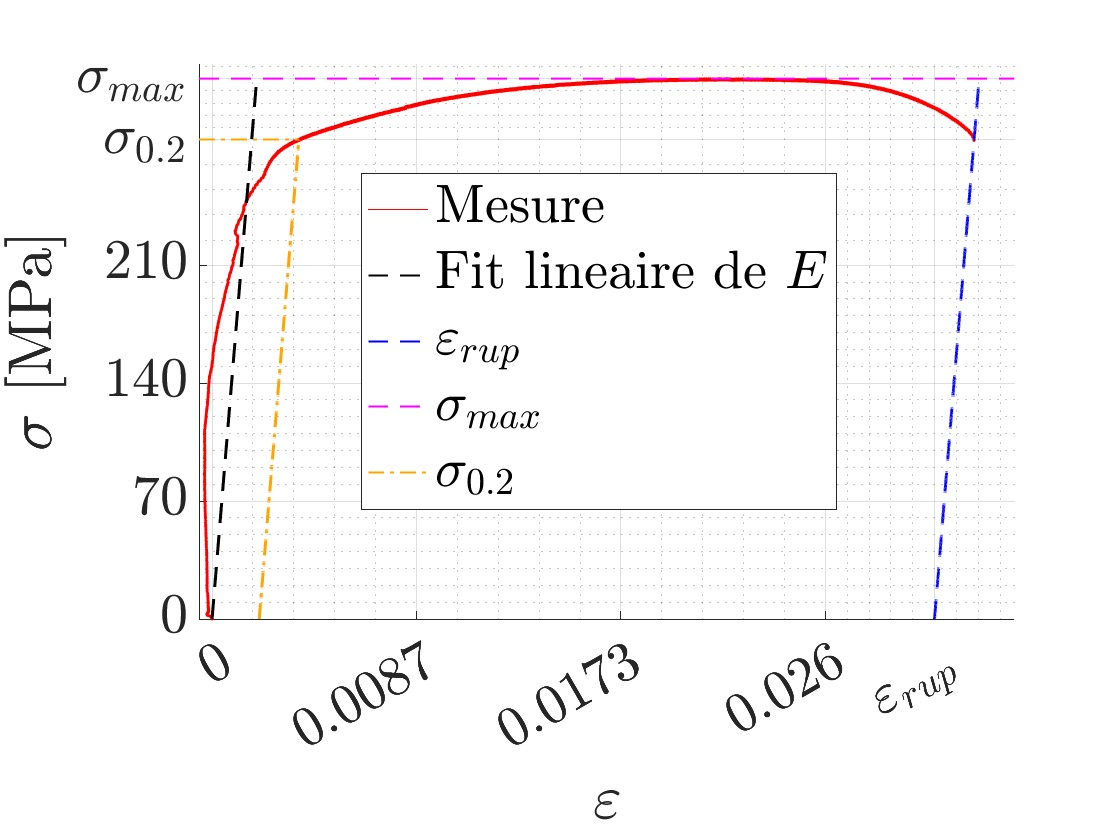
\includegraphics[width=0.45\textwidth]{GRAPHES/Graphe_2.jpg}
    \captionsetup{justification=centering}
    \caption{Courbe de traction du deuxième échantillon non traité}
    \label{fig10}
\end{figure}

\end{document}
